\section{Additional Benchmark Details}
\label{app:benchmark}


\subsection{Benchmark and Data Flow}

Figure~\ref{fig:data-pipeline} details the preprocessing path introduced in Figure~\ref{fig:thesis-overview}. Combined pools the two source databases. It is not an external cohort. The varying unit includes objective-specific masks, auxiliary modules, and compute.

\begin{figure*}[p]
\floatconts{fig:data-pipeline}
{\caption{Data pipeline. RICU supplies concept-specific harmonization and hourly aggregation. SLICES applies cohort and feature filters and forms values, masks, and labels. Patient assignment precedes task-specific null-label filtering. Normalization uses observed training cells, followed by zero filling with the observation mask retained. Event rows are illustrative.}}
{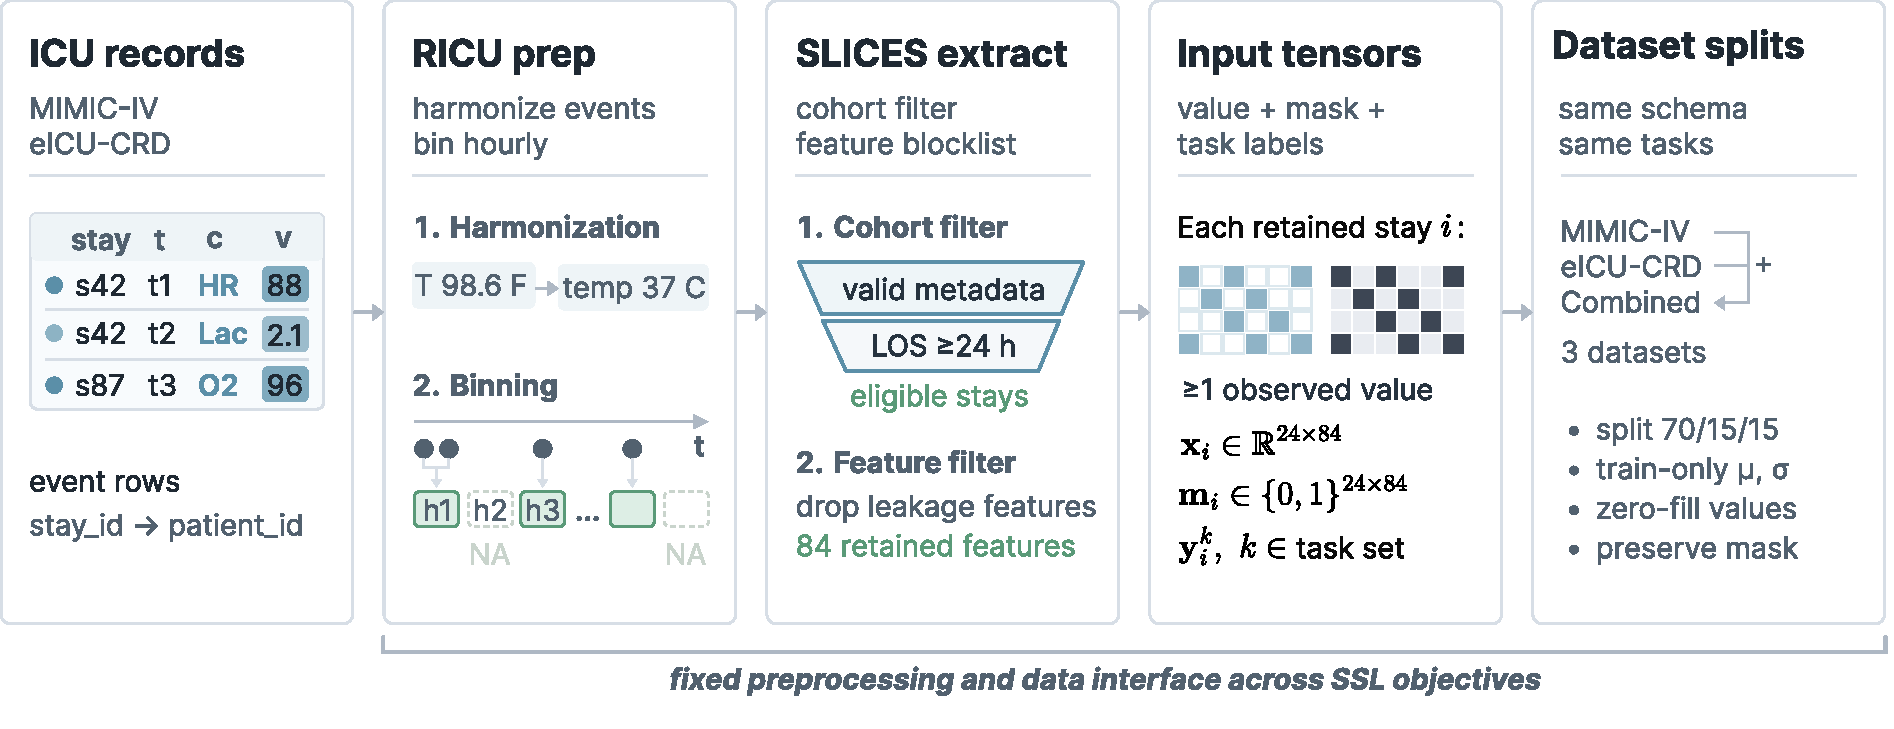
\includegraphics[width=\textwidth]{diagrams/fig02-data-pipeline.pdf}}
\end{figure*}

\begin{figure*}[p]
\floatconts{fig:encoder-tokenization}
{\caption{Shared hourly tokenization and encoder. Values and masks form 168 inputs per hour, projected to 64 dimensions. Empty hours are excluded from attention and losses. SSL uses timestep outputs, with objective-specific pooling for contrastive learning. Downstream heads mean-pool valid hours.}}
{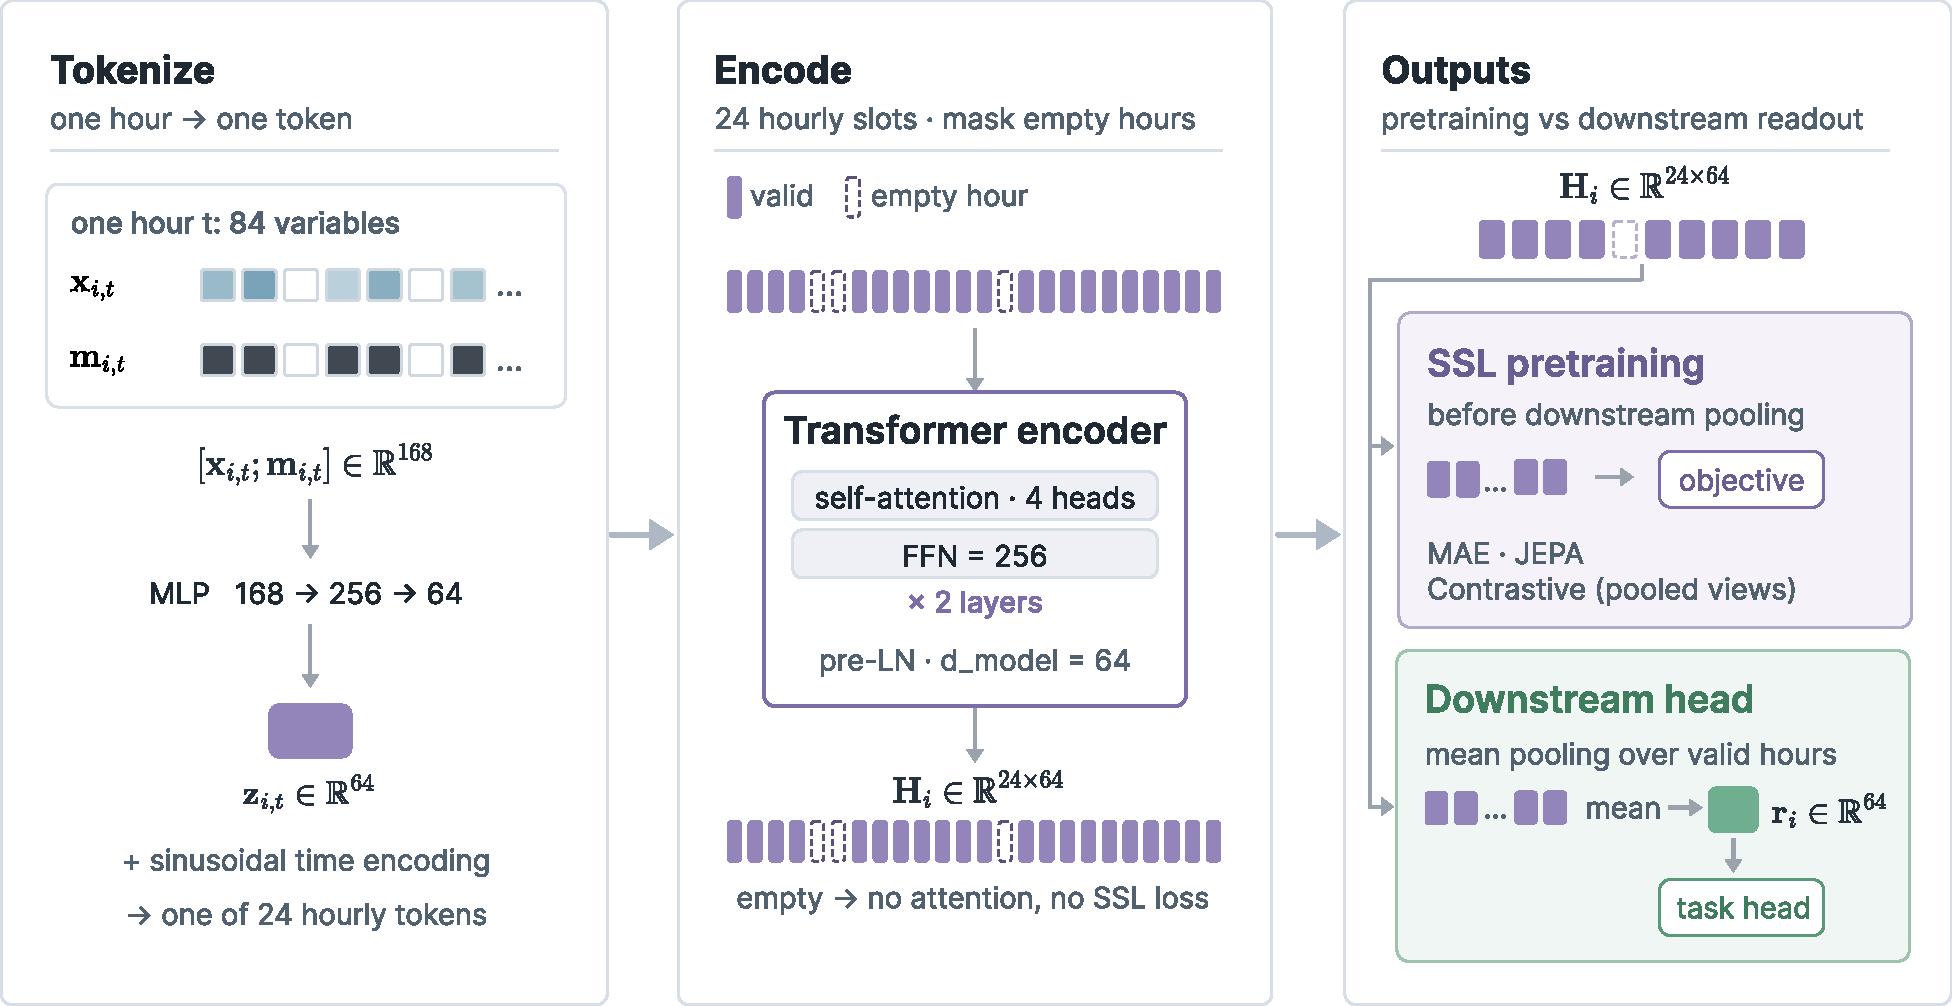
\includegraphics[width=\textwidth]{diagrams/fig03-encoder-tokenization.pdf}}
\end{figure*}

\subsection{Downstream Protocols}

Figure~\ref{fig:protocol-ab} separates frozen probing from full fine-tuning. Both use the same final pretraining encoder but differ in trainable scope, head capacity, learning rate, and epoch cap. These are two evaluation protocols, not a freeze-only ablation. The separate checkpoint diagnostic changes the SSL encoder selection policy only within its stated scope.

\begin{figure*}[p]
\floatconts{fig:protocol-ab}
{\caption{Reference downstream protocols. The displayed 50 and 100 epochs are maximum budgets. Validation patience is ten epochs. Protocol A (frozen probing) trains a linear head. Protocol B (full fine-tuning) adapts the encoder and a width-64 MLP head. Validation selects each downstream checkpoint before one test evaluation. Both start from final-epoch SSL weights.}}
{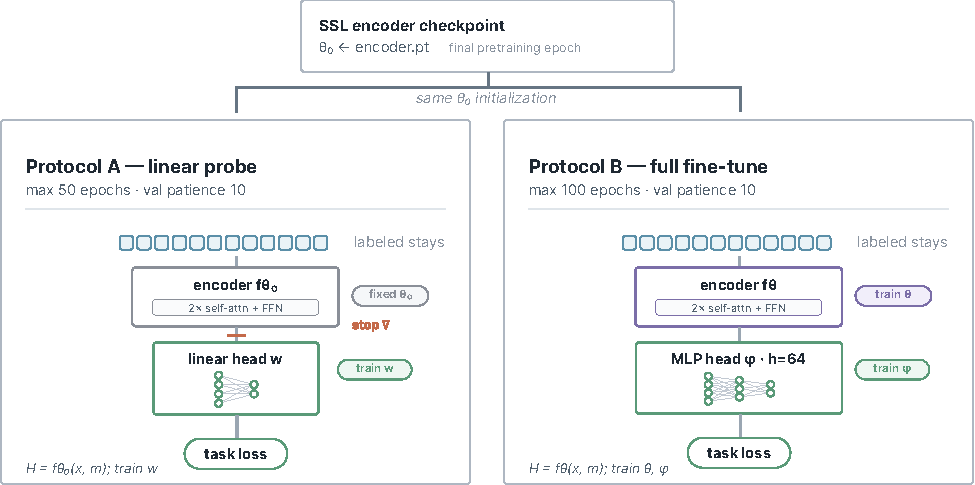
\includegraphics[width=\textwidth]{diagrams/fig05-protocol-ab.pdf}}
\end{figure*}

\subsection{Task Definitions and Test Support}

Tables~\ref{tab:task-definitions} and~\ref{tab:test-support} give the target rules and exported test support. Twenty-four-hour mortality and remaining LOS are fixed-window analogues of the decompensation and length-of-stay tasks of \citet{harutyunyan2019multitask}, and mortality, AKI, and LOS appear in YAIB \citep{van_de_water2024yaib}. The four endpoints span 1.6\%--20.3\% prevalence, two horizons, a laboratory-defined label with structured missing labels, and a continuous target. The SSL ordering is uniform for frozen classification but not for fine-tuning or against supervised and classical baselines, so these differences matter for the comparison.

\begin{table*}[htbp]
\floatconts
  {tab:task-definitions}
  {\caption{Downstream task contract. All tasks use hours 0--24 as model input.}}
  {\scriptsize
  \begin{tabular}{>{\raggedright\arraybackslash}p{.12\textwidth}>{\raggedright\arraybackslash}p{.12\textwidth}>{\raggedright\arraybackslash}p{.22\textwidth}>{\raggedright\arraybackslash}p{.25\textwidth}l}
  \toprule
  Task & Horizon after input & Target & Null-label rule & Primary metric \\
  \midrule
  24h mortality & hours 24--48 & death in forward day & death in hours 0--24 & AUPRC \\
  Hosp. mortality & after hour 24 & death before discharge & death in hours 0--24 & AUPRC \\
  AKI & hours 24--48 & creatinine-defined KDIGO~stage~$\geq$1 & missing baseline/forward evidence & AUPRC \\
  Remaining LOS & after hour 24 & ICU LOS minus one day, clipped at 0 & none & Absolute error (days) \\
  \bottomrule
  \end{tabular}}
\end{table*}

\begin{table*}[htbp]
\floatconts
  {tab:test-support}
  {\caption{Mean test support across the five patient splits. Positive counts and prevalence apply to classification tasks.}}
  {\scriptsize
  \begin{tabular}{llrrr}
\toprule
Data & Task & Test samples & Positive & Prevalence \\
\midrule
Combined & 24h mortality & 30,863.4 & 492.4 & 0.0160 \\
Combined & Hospital mortality & 30,869.0 & 3,135.8 & 0.1016 \\
Combined & AKI & 21,724.0 & 3,565.2 & 0.1641 \\
Combined & Remaining LOS & 31,092.2 & -- & -- \\
eICU-CRD & 24h mortality & 19,788.6 & 315.2 & 0.0159 \\
eICU-CRD & Hospital mortality & 19,788.6 & 1,823.8 & 0.0922 \\
eICU-CRD & AKI & 13,297.4 & 1,850.0 & 0.1391 \\
eICU-CRD & Remaining LOS & 19,966.4 & -- & -- \\
MIMIC-IV & 24h mortality & 11,150.0 & 185.4 & 0.0166 \\
MIMIC-IV & Hospital mortality & 11,157.0 & 1,310.0 & 0.1174 \\
MIMIC-IV & AKI & 8,423.2 & 1,710.6 & 0.2031 \\
MIMIC-IV & Remaining LOS & 11,194.8 & -- & -- \\
\bottomrule
\end{tabular}
}
\end{table*}

\subsection{Objective and Downstream Configuration}
\label{app:config}

\begin{table}[!htbp]
\floatconts
  {tab:pretraining}
  {\caption{Core pretraining contract. Ratio is the configured timestep-mask ratio. All rows use AdamW, batch size 256, 100 epochs, and the same transferred encoder.}}
  {\scriptsize
  \begin{tabular}{llll}
  \toprule
  Objective & Masking & Target & Ratio \\
  \midrule
  \MAE{} & random hours & observed values & .5 \\
  \JEPA{} & $\leq3$ blocks & target embeddings & .5 \\
  Contrastive & two views & view agreement & .5 \\
  \bottomrule
  \end{tabular}}
\end{table}

\begin{table*}[htbp]
\floatconts
  {tab:objective-details}
  {\caption{Objective-specific modules and transferred capacity. Shared settings are listed in Section~\ref{sec:setup}.}}
  {\scriptsize
  \begin{tabular}{llllrr}
  \toprule
  Objective & Geometry & Learning target & Auxiliary module & Trainable & Transferred \\
  \midrule
  \MAE{} & random masked hours & observed normalized cells & Transformer decoder & 269,460 & 159,808 \\
  \JEPA{} & up to three masked blocks & EMA target embeddings & predictor + target encoder & 189,440 & 159,808 \\
  Contrastive & complementary views & instance agreement & projection MLP & 193,408 & 159,808 \\
  \bottomrule
  \end{tabular}}
\end{table*}

\paragraph{Development and test-set use.}
Every downstream run reports test metrics automatically, and the pipeline was run end to end a few times before the final rerun. Those earlier passes exposed defects that were fixed: an AKI label that overlapped the input window (detected through test AUROC above .97 for every method), mislabeled boundary cases in the mortality labels, and input features derived from future treatment durations. The test metrics we saw therefore came largely from earlier benchmark versions with different labels or inputs. Pretraining does not read the test partition, checkpoints are selected on validation metrics, and each run scores the test partition once after selection. The recorded objective-specific changes responded to label-free pretraining diagnostics: a rising JEPA loss with low representation spread, and a contrastive pretext task that was solved almost perfectly. Settings shaped by downstream comparisons are shared by all three objectives: input representation, encoder, one pretraining learning rate, one mask ratio, and one downstream recipe that the supervised Transformer also uses. Across the tested learning rates and mask ratios, mean test AUPRC moves by at most .018 within a sweep and .020 within an objective (\tableref{tab:hp}).

The \JEPA{} target encoder adds a non-trainable 159,808-parameter copy. Its EMA coefficient increases linearly from .999 to 1.0. The predictor has width 32, two layers, four heads, and feed-forward width 128. The contrastive projection has hidden width 256 and output width 64. All auxiliary modules are discarded before downstream evaluation.

\subsection{Retained Features and Preprocessing}

The ordered 84 RICU concept identifiers below define the model schema, not a claim that each is observed in both sources. Source-specific missingness remains explicit. Extraction uses RICU 0.6.3 concept definitions and unit conversions, requested at one-hour intervals. Concept-specific aggregation is inherited from RICU. Python tensorization neither quantizes values nor forward-fills across hours. It uses the observed training-partition mean and sample SD per feature. SD is floored at $10^{-6}$. Features absent in training retain a zero mean and unit SD. Missing values become zero after normalization. Low-label subsets retain the full training-partition normalizer. The code repository includes extraction scripts and the complete input blocklist, including direct LOS, future vasopressor-duration, and derived score features.

\begin{quote}\footnotesize
\texttt{abx}, \texttt{adh\_rate}, \texttt{alb}, \texttt{alp}, \texttt{alt}, \texttt{ast}, \texttt{avpu}, \texttt{basos}, \texttt{be}, \texttt{bicar}, \texttt{bili}, \texttt{bili\_dir}, \texttt{bnd}, \texttt{bun}, \texttt{ca}, \texttt{cai}, \texttt{ck}, \texttt{ckmb}, \texttt{cl}, \texttt{cort}, \texttt{crea}, \texttt{crp}, \texttt{dbp}, \texttt{dex}, \texttt{dobu\_rate}, \texttt{dopa\_rate}, \texttt{egcs}, \texttt{eos}, \texttt{epi\_rate}, \texttt{esr}, \texttt{etco2}, \texttt{ett\_gcs}, \texttt{fgn}, \texttt{fio2}, \texttt{glu}, \texttt{hba1c}, \texttt{hbco}, \texttt{hct}, \texttt{hgb}, \texttt{hr}, \texttt{inr\_pt}, \texttt{ins}, \texttt{k}, \texttt{lact}, \texttt{lymph}, \texttt{map}, \texttt{mch}, \texttt{mchc}, \texttt{mcv}, \texttt{mech\_vent}, \texttt{methb}, \texttt{mg}, \texttt{mgcs}, \texttt{na}, \texttt{neut}, \texttt{norepi\_rate}, \texttt{o2sat}, \texttt{pco2}, \texttt{ph}, \texttt{phn\_rate}, \texttt{phos}, \texttt{plt}, \texttt{po2}, \texttt{pt}, \texttt{ptt}, \texttt{rass}, \texttt{rbc}, \texttt{rdw}, \texttt{resp}, \texttt{samp}, \texttt{sao2}, \texttt{sbp}, \texttt{spo2}, \texttt{supp\_o2}, \texttt{tco2}, \texttt{temp}, \texttt{tgcs}, \texttt{tnt}, \texttt{tri}, \texttt{urine}, \texttt{vent\_end}, \texttt{vent\_start}, \texttt{vgcs}, \texttt{wbc}.
\end{quote}

\subsection{Exact Losses and Baseline Configuration}

MAE minimizes squared reconstruction error averaged over observed feature cells at masked non-empty hours. JEPA uses elementwise squared error between predictions and layer-normalized stop-gradient target embeddings, averaged across valid target dimensions/hours. Its EMA coefficient rises from .999 to 1.0. EMA and target normalization are not evidence of collapse prevention. Core contrastive learning uses cosine similarity between normalized projected stay vectors. Each of the $2B$ view embeddings has its paired view as positive and the other non-self batch views in an NT-Xent denominator, at temperature .07. Losses differ in target space and reduction unit.

Binary mortality and AKI use two-logit cross entropy with label smoothing .1 and class weights $w_c=\sqrt{n/(2n_c)}$ from the labeled training subset. They are classification tasks, not time-to-event regression. LOS uses untransformed remaining days, squared-error training loss, and absolute-error validation/test evaluation. The constant median is the empirical training-label median evaluated on the test labels. It is not fitted on the test set.

GRU-D has hidden width 64, one recurrent layer, dropout .1, learned input/hidden decay, and the full-fine-tuning head and schedule. XGBoost receives eight summaries per variable: observed mean, SD, minimum, maximum, first, last, count, and fraction, for 672 inputs. It uses at most 1,000 trees, depth 6, learning rate .1, row/column subsampling .8, minimum child weight 1, and validation patience 20. Classification uses the native negative/positive class ratio and validation \texttt{aucpr}. Regression uses the squared-error objective and validation \texttt{mae}. These differ from neural weighting and average-precision implementation. All test AUPRC values use the shared evaluation definition. Exported per-run scientific configurations, rather than current defaults, are the reproduction reference.

\subsection{Full Baseline Matrix}

Table~\ref{tab:baseline-full} reports all full-label contextual baseline comparisons.

\begin{table*}[htbp]
\floatconts
  {tab:baseline-full}
  {\caption{Full-data contextual baselines and the best SSL mean. Classification rows report AUPRC (higher is better). LOS rows report absolute error in days (lower is better). Bold marks the best unrounded mean per row. All entries average five seeds.}}
  {\scriptsize
  \begin{tabular}{llrrrrl}
\toprule
Data & Endpoint & GRU-D & XGBoost & Supervised & Best SSL & SSL method \\
\midrule
Combined & 24h mortality & \textbf{0.422} & 0.374 & 0.389 & 0.409 & MAE \\
Combined & Hospital mortality & 0.527 & 0.525 & 0.518 & \textbf{0.531} & MAE \\
Combined & AKI & 0.630 & \textbf{0.668} & 0.652 & 0.626 & JEPA \\
Combined & Remaining LOS & 2.174 & 2.340 & 2.190 & \textbf{2.118} & MAE \\
eICU-CRD & 24h mortality & \textbf{0.397} & 0.315 & 0.351 & 0.377 & MAE \\
eICU-CRD & Hospital mortality & 0.484 & 0.482 & 0.474 & \textbf{0.495} & MAE \\
eICU-CRD & AKI & 0.510 & \textbf{0.569} & 0.554 & 0.519 & MAE \\
eICU-CRD & Remaining LOS & 2.003 & 2.163 & 1.997 & \textbf{1.964} & MAE \\
MIMIC-IV & 24h mortality & \textbf{0.480} & 0.402 & 0.449 & 0.456 & Contrastive \\
MIMIC-IV & Hospital mortality & 0.577 & 0.577 & 0.565 & \textbf{0.579} & MAE \\
MIMIC-IV & AKI & 0.661 & \textbf{0.729} & 0.693 & 0.667 & MAE \\
MIMIC-IV & Remaining LOS & 2.394 & 2.613 & 2.397 & \textbf{2.359} & Contrastive \\
\bottomrule
\end{tabular}
}
\end{table*}
